\documentclass[11pt]{article}

\usepackage[margin=1in]{geometry}
\usepackage{graphicx}
\usepackage{booktabs}
\usepackage{xcolor}
\usepackage{amsmath}
\usepackage{amssymb}
\usepackage{caption}
\usepackage{float}
% placeins unavailable on this system; with [H] floats are placed in-line, so
% a no-op \FloatBarrier suffices to keep each figure with its paragraph.
\providecommand{\FloatBarrier}{}
\usepackage[colorlinks=true,linkcolor=accent,urlcolor=accent,citecolor=accent]{hyperref}

% --- colours ---
\definecolor{accent}{RGB}{20,90,150}
\definecolor{accentlight}{RGB}{232,240,248}
\definecolor{rulegray}{RGB}{120,120,120}

% --- section heading styling: a touch of colour + a rule ---
% (titlesec/sectsty unavailable; redefine \section/\subsection via \@startsection)
\makeatletter
\renewcommand\section{\@startsection{section}{1}{\z@}%
  {-3.5ex \@plus -1ex \@minus -.2ex}%
  {2.3ex \@plus.2ex}%
  {\normalfont\Large\bfseries\color{accent}}}
\renewcommand\subsection{\@startsection{subsection}{2}{\z@}%
  {-3.25ex\@plus -1ex \@minus -.2ex}%
  {1.5ex \@plus .2ex}%
  {\normalfont\large\bfseries\color{accent}}}
\makeatother

\captionsetup{font=small,labelfont={bf,color=accent}}
\setlength{\parskip}{0.4em}
\setlength{\parindent}{0pt}

% --- headline box: framed minipage fallback (tcolorbox/mdframed unavailable) ---
\newcommand{\headlinebox}[1]{%
  \begin{center}
  \setlength{\fboxsep}{12pt}%
  \setlength{\fboxrule}{1.2pt}%
  \fcolorbox{accent}{accentlight}{%
    \begin{minipage}{0.92\textwidth}
    #1
    \end{minipage}}%
  \end{center}}

\begin{document}

The two scan modes give two distinct notions of a floor. The \emph{typical}
(median) floor is where the bulk of anarchic points become excluded; the
\emph{existence} (best/tuned) floor is where even the single best-aligned point
crosses the bound. Flavor constraints separate the two by orders of magnitude
(they are tunable); the oblique $S,T,U$ constraint does not (it has no Yukawa
freedom).

\begin{center}
\small
\setlength{\tabcolsep}{5pt}
\begin{tabular}{@{}llll@{}}
\toprule
\textbf{Constraint} & \textbf{Typical (median)} & \textbf{Existence (best/tuned)} & \textbf{Tunable?} \\
\midrule
$\varepsilon_K$            & ${\sim}30$~TeV (anarchic) & ${\lesssim}1$~TeV & yes (align $\mathrm{Im}\,M_{12}\!\to\!0$) \\
$\Delta m_d$ ($B_d$)       & few TeV & ${\lesssim}1$~TeV & yes \\
$\Delta m_s$ ($B_s$)       & few TeV & ${\lesssim}1$~TeV & yes \\
$D^0$                      & low & ${\lesssim}1$~TeV & yes \\
$\Delta m_K$               & low & ${\lesssim}3$~TeV & yes \\
$Z\to b\bar b$ (T010)      & ${\sim}5$~TeV & ${\sim}4.6$~TeV & no (gauge-dominated; $c_{Q_3}$ pinned by $m_t$) \\
$S,T,U$ (EW001)            & ${\sim}20$~TeV & ${\sim}18\text{--}20$~TeV & no (no Yukawa dependence) \\
\midrule
\textbf{COMBINED}          & \textbf{${\sim}30$~TeV} ($\varepsilon_K$) & \textbf{${\sim}18\text{--}20$~TeV} ($S,T,U$) & \\
\bottomrule
\end{tabular}
\end{center}

\FloatBarrier


% ---- STU ----
\subsection*{$S,T,U$ oblique: Casagrande et al.\ 0807.4937, Fig.~4 \quad(paper left, ours right)}
\begin{figure}[H]
\centering
\begin{minipage}[c]{0.49\textwidth}\centering
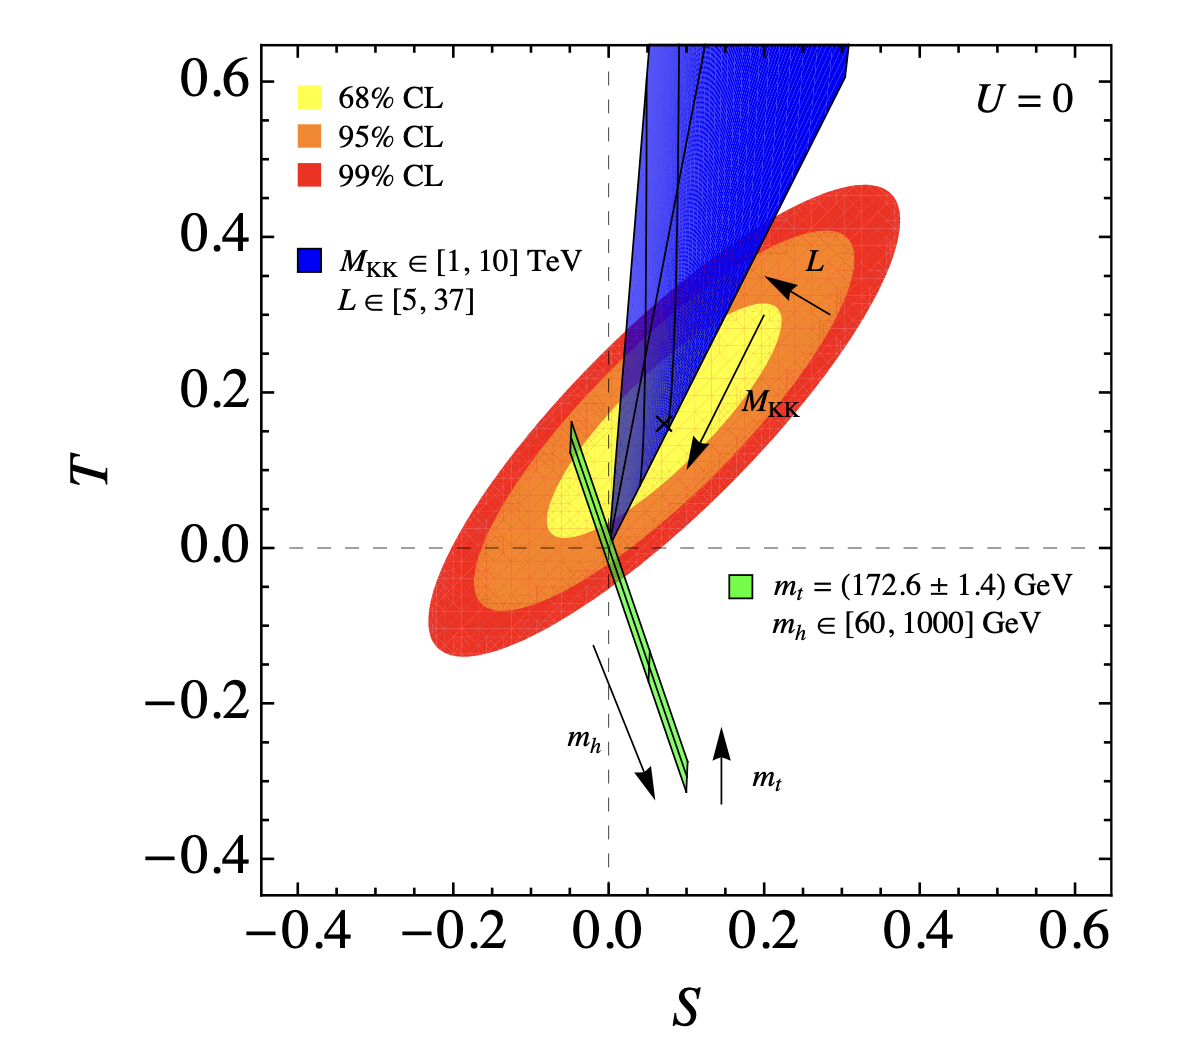
\includegraphics[width=\linewidth]{figures/paper_STU.png}
\end{minipage}\hfill
\begin{minipage}[c]{0.49\textwidth}\centering
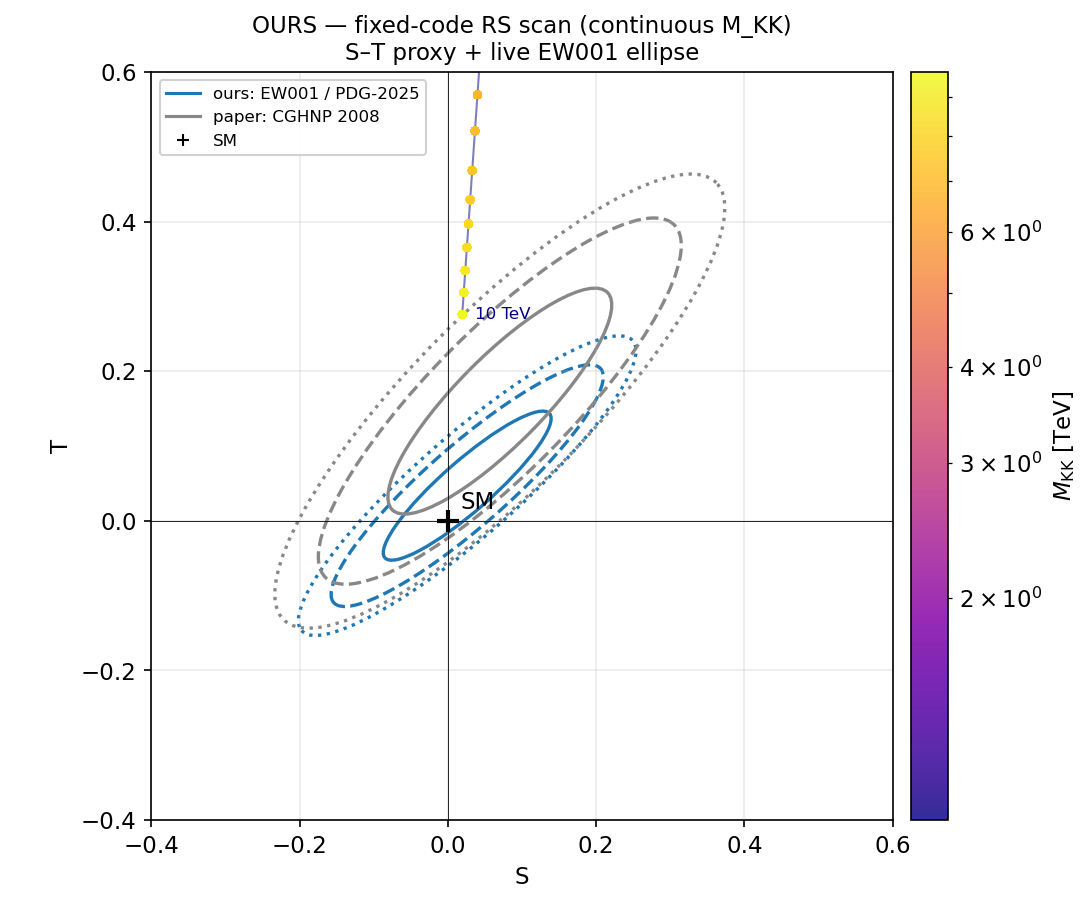
\includegraphics[width=\linewidth]{figures/ours_STU.png}
\end{minipage}
\caption{The $S$--$T$ plane: paper (left) vs.\ ours (right). Minimal RS sweeps a
wedge over $M_{KK}$ ($1\to10$~TeV) and warp volume $L$ against the CL ellipses.}
\end{figure}


\FloatBarrier

% ---- Zbb_gLgR ----
\subsection*{$Z\to b\bar b$ couplings: Casagrande et al.\ 0807.4937, Fig.~8 \quad(paper left, ours right)}
\begin{figure}[H]
\centering
\begin{minipage}[c]{0.49\textwidth}\centering
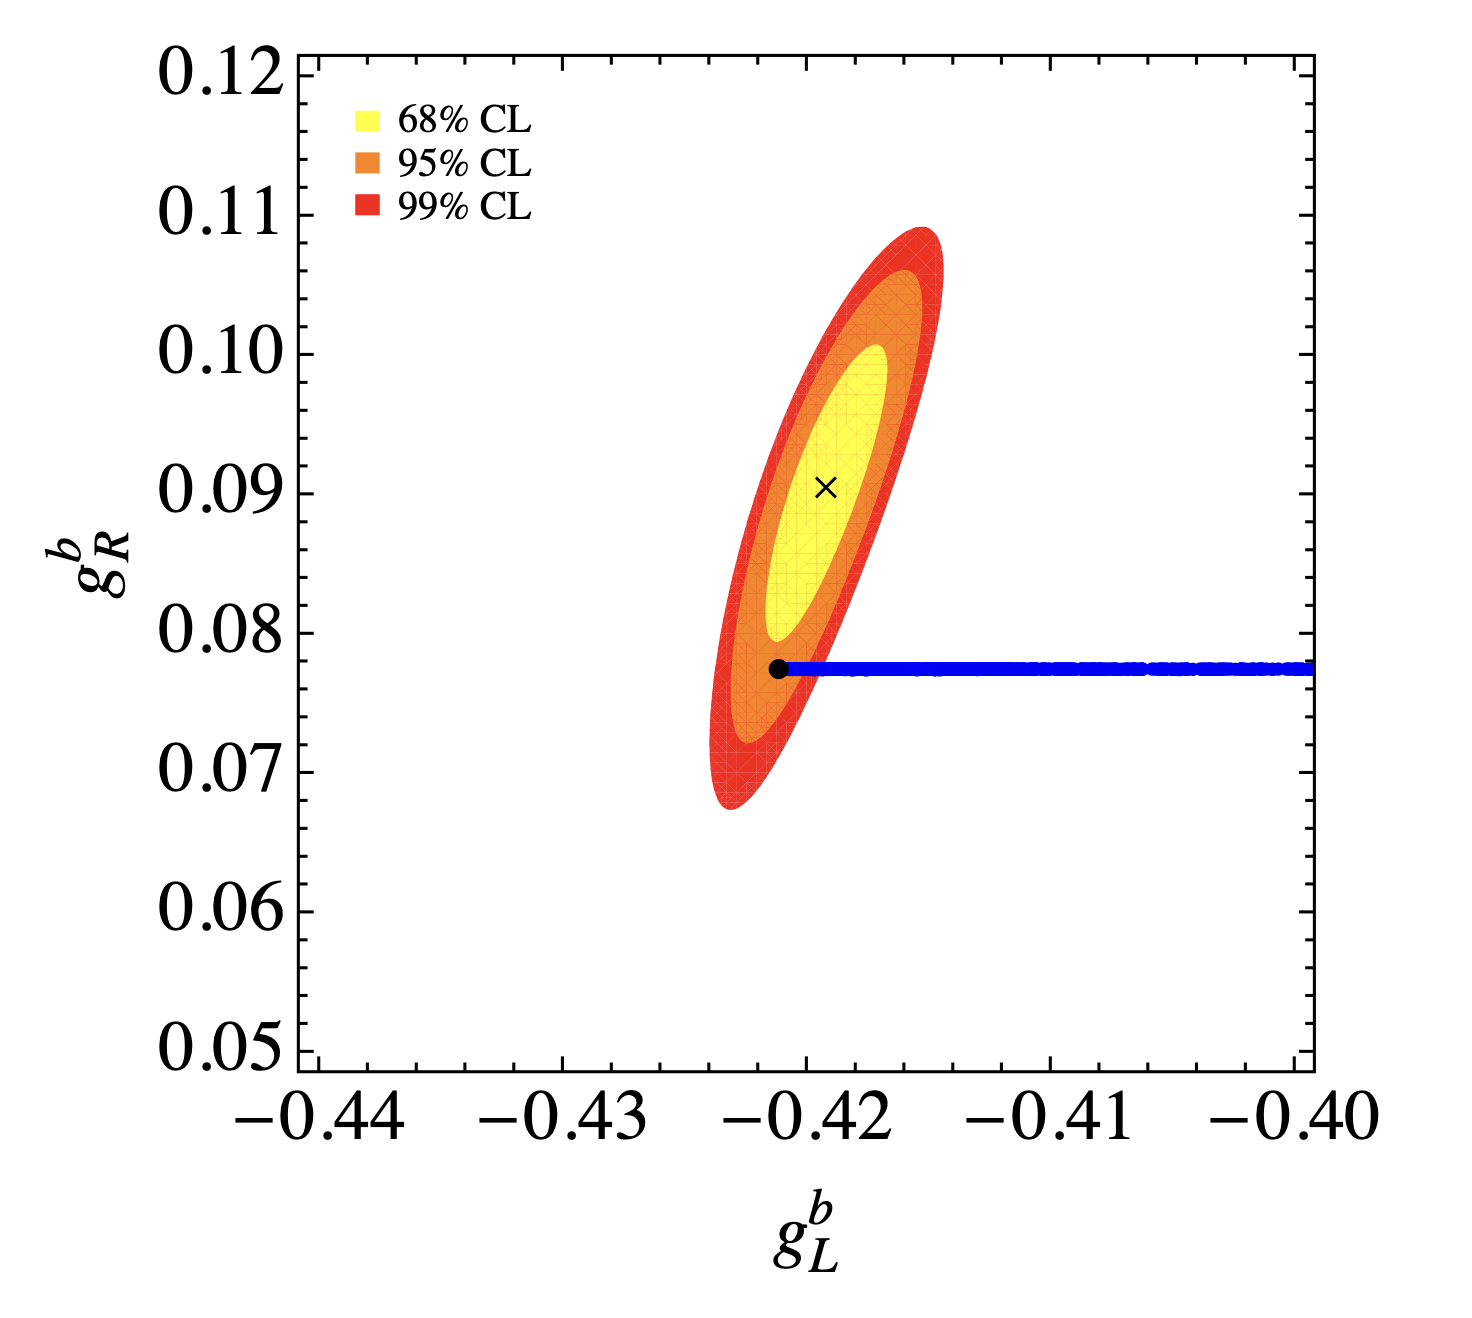
\includegraphics[width=\linewidth]{figures/paper_Zbb_gLgR.png}
\end{minipage}\hfill
\begin{minipage}[c]{0.49\textwidth}\centering
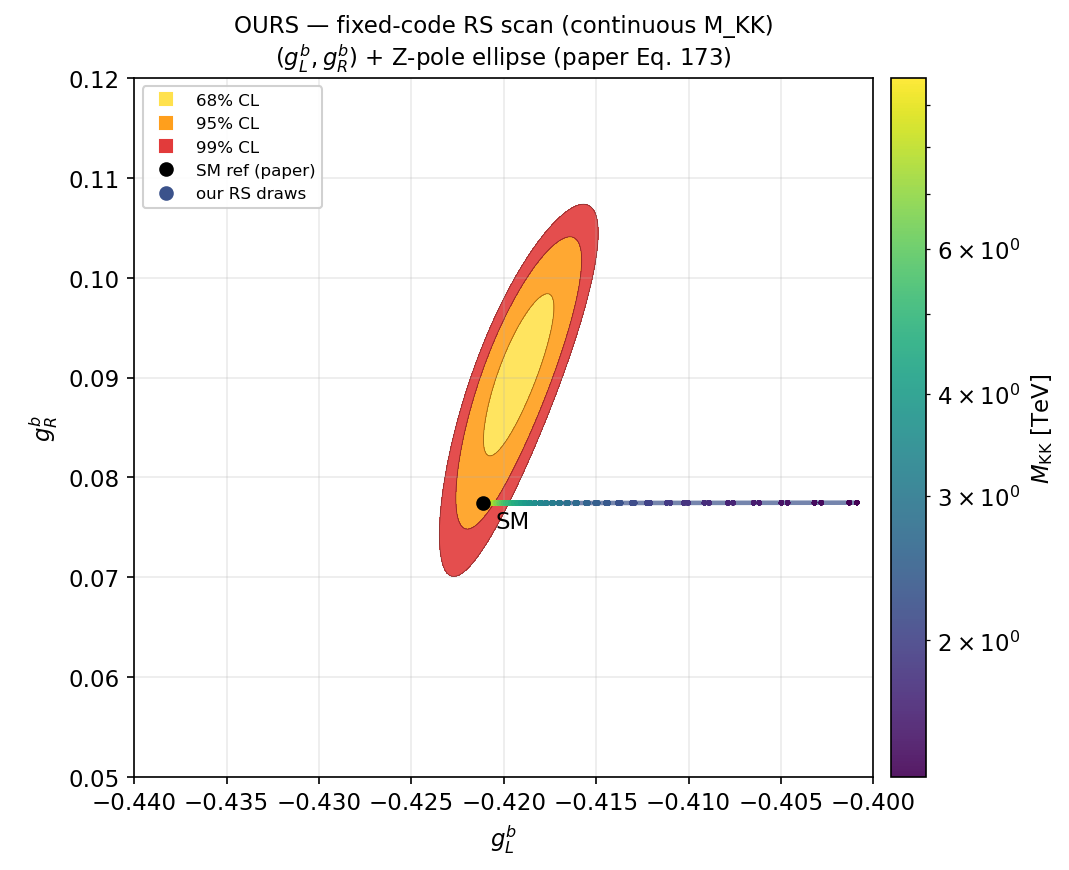
\includegraphics[width=\linewidth]{figures/ours_Zbb_gLgR.png}
\end{minipage}
\caption{The $(g_L^b, g_R^b)$ plane: paper (left) vs.\ ours (right), with the
$Z$-pole CL ellipses and the SM point.}
\end{figure}


\FloatBarrier

% ---- epsK_cloud ----
\subsection*{$\varepsilon_K$: Bauer et al.\ 0912.1625, Fig.~4 \quad(paper left, ours right)}
\begin{figure}[H]
\centering
\begin{minipage}[c]{0.49\textwidth}\centering
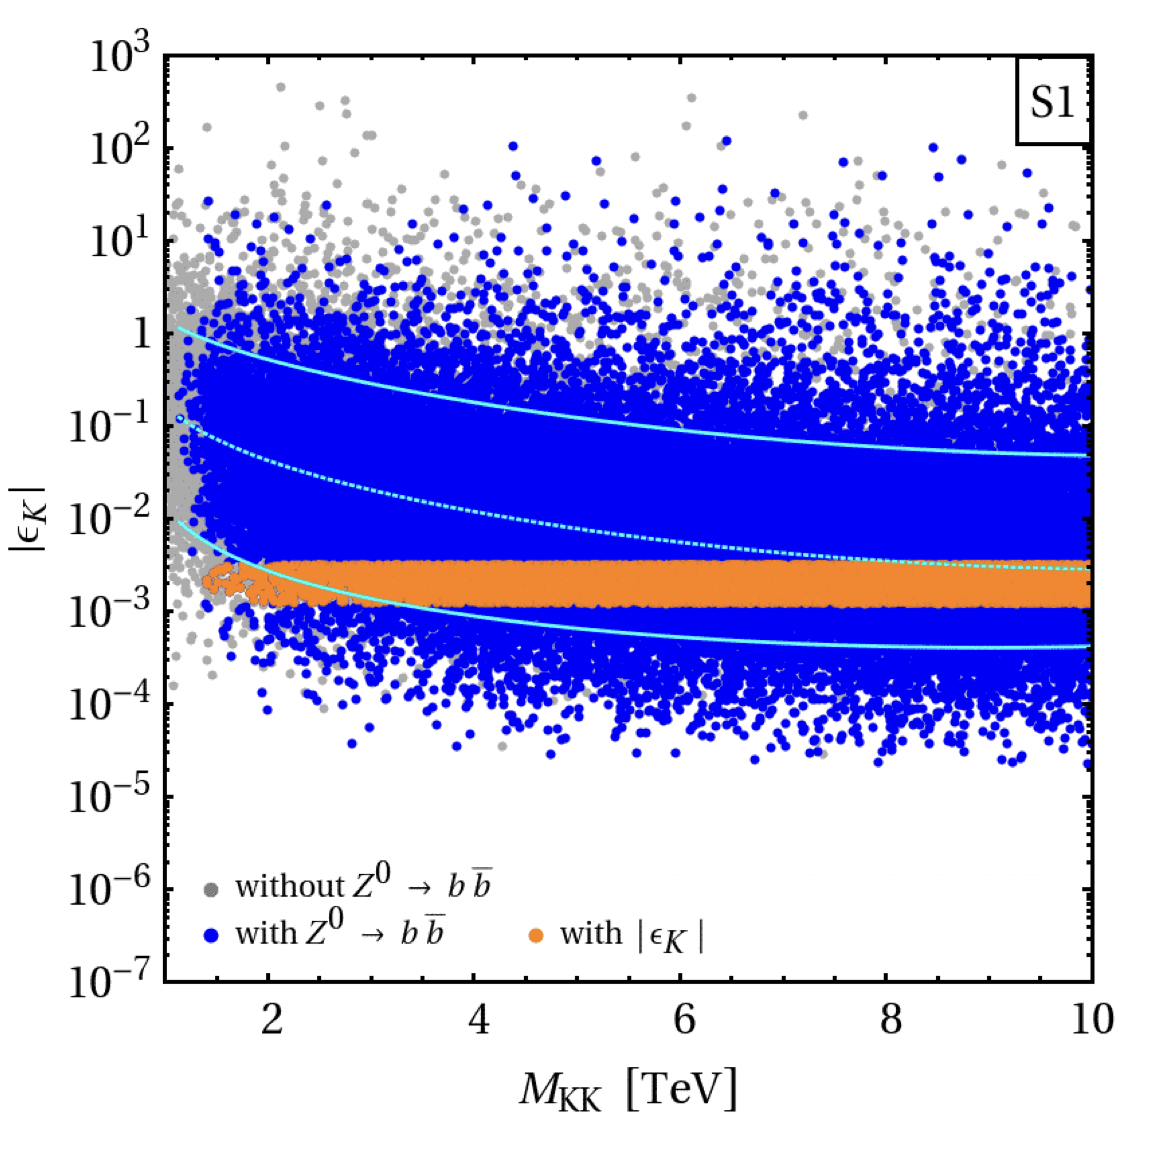
\includegraphics[width=\linewidth]{figures/paper_epsK.png}
\end{minipage}\hfill
\begin{minipage}[c]{0.49\textwidth}\centering
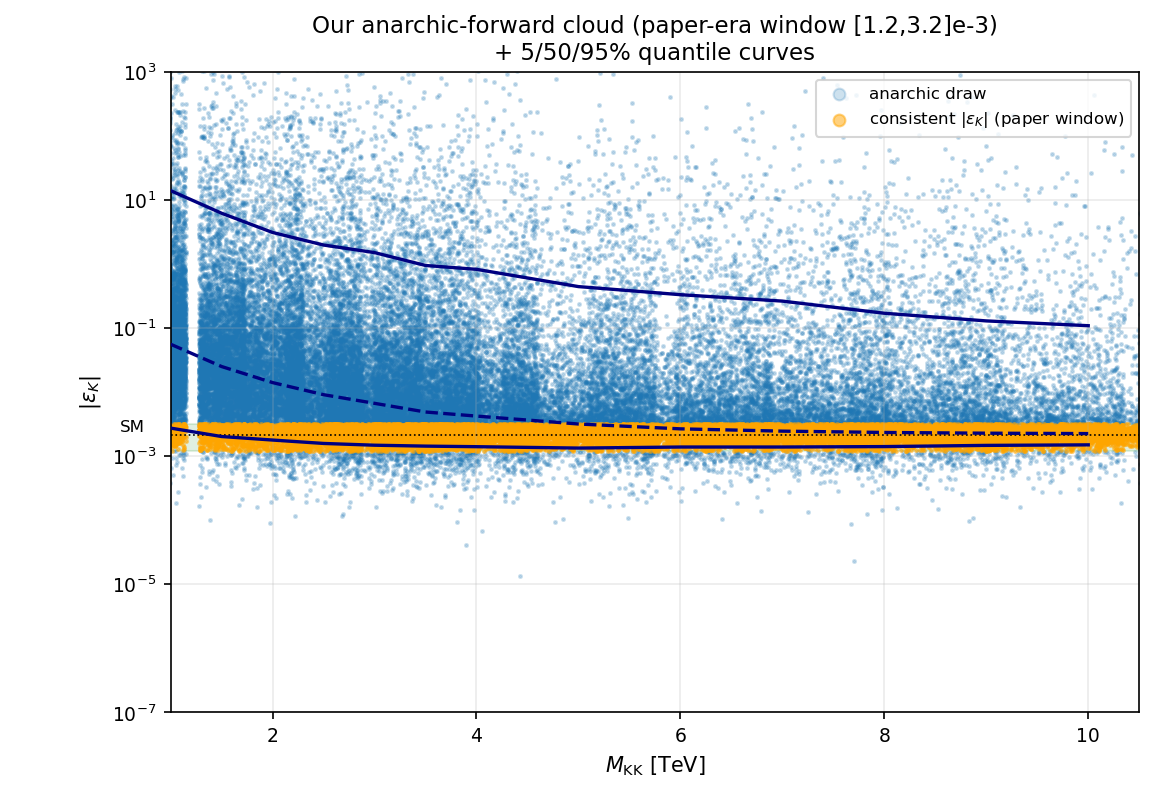
\includegraphics[width=\linewidth]{figures/ours_epsK.png}
\end{minipage}
\caption{Anarchic $|\varepsilon_K|$ vs.\ $M_{KK}$: paper (left) vs.\ ours (right),
with 5/50/95\% quantile curves. Paper scatters anarchic Yukawas; we reproduce the
fat cloud in anarchic-forward mode.}
\end{figure}


\end{document}
